\documentclass{beamer}

\mode<presentation>
{
  \usetheme{CambridgeUS}
  \usecolortheme{seagull}
  \setbeamercovered{transparent}
}

\usepackage[english]{babel}
\usepackage[latin1]{inputenc}
\usepackage{times}
\usepackage[T1]{fontenc} 
% Or whatever. Note that the encoding and the font should match. If T1
% does not look nice, try deleting the line with the fontenc.
\usepackage{amsmath}

\newcommand{\linespace}{\vskip 0.25cm}

\definecolor{MyForestGreen}{rgb}{0,0.7,0} 
\newcommand{\tableemph}[1]{{#1}}
\newcommand{\tablewin}[1]{\tableemph{#1}}
\newcommand{\tablemid}[1]{\tableemph{#1}}
\newcommand{\tablelose}[1]{\tableemph{#1}}

\definecolor{MyLightGray}{rgb}{0.6,0.6,0.6}
\newcommand{\tabletie}[1]{\color{MyLightGray} {#1}}

% The text in square brackets is the short version of your title and will be used in the
% header/footer depending on your theme.
\title[Concurrent Compaction in JVM GC]{Concurrent Compaction in JVM Garbage Collection}

% Sub-titles are optional - uncomment and edit the next line if you want one.
% \subtitle{Why does sub-tree crossover work?} 

% The text in square brackets is the short version of your name(s) and will be used in the
% header/footer depending on your theme.
\author[Jacob Opdahl]{Jacob P. Opdahl}


% The text in square brackets is the short version of your institution and will be used in the
% header/footer depending on your theme.
\institute[UMM]
{
  University of Minnesota, Morris \\[\baselineskip]
  \emph{opdah023@morris.umn.edu}
}

% The text in square brackets is the short version of the date if you need that.
\date[December 5, 2015] % (optional)
{December 5, 2015}

% Delete this, if you do not want the table of contents to pop up at
% the beginning of each subsection:
\AtBeginSection[]
{
  \begin{frame}<beamer>
    \frametitle{Outline}
    \tableofcontents[currentsection, hideothersubsections]
  \end{frame}
}

%\AtBeginSubsection[]
%{
%\begin{frame}<beamer>
%    \frametitle{Outline}
%    \tableofcontents[currentsection, currentsubsection]
%  \end{frame}
%}

\begin{document}

\begin{frame}
  \titlepage
\end{frame}

% For a 20-25 minute senior seminar talk you probably want something like:
% - Two or three major sections (other than the summary).
% - At *most* three subsections per section.
% - Talk about 30s to 2min per frame. So there should probably be between
%   15 and 30 frames, all told.



\section*{Overview}

\subsection*{Introduction}

\begin{frame}

\frametitle{Automatic Memory Management}

Implicit allocation and deallocation of memory

\linespace
\linespace

Languages: Java, C\#, Python, and more
\begin{itemize}
\item We focus on the Java Virtual Machine and languages it supports
\end{itemize}

\linespace
\linespace

Abstracts details away from the developer

\linespace

\begin{center}

\includegraphics[width=.3\textwidth]{Illustrations/garbage.jpg}
\end{center}

\end{frame}

\begin{frame}

\frametitle{Implicit Deallocation}

Memory is a finite resource

\linespace
\linespace

\emph{Garbage}: objects that are no longer reachable

\linespace
\linespace

\emph{Garbage Collection (GC)}: detecting and removing garbage

\linespace
\linespace
\linespace

\begin{center}

\includegraphics[width=.3\textwidth]{Illustrations/garbage.jpg}
\end{center}

\end{frame}

\begin{frame}

\begin{columns}
\begin{column}{0.65\textwidth}

\frametitle{Stopping the World}

GC requires processing resources

\linespace
\linespace

When only one processor is used, collectors \emph{stop the world}
% Need to get across that this can still be ueful.

\linespace
\linespace

Problem: applications today are subjected to increasing pauses
\begin{itemize}
\item More memory
\item More strenuous applications
\end{itemize}

\linespace
\linespace

Use parallel processing to solve!
\end{column}
\begin{column}{0.35\textwidth}

\begin{center}

\includegraphics[width=.8\textwidth]{Illustrations/meme.jpg}
\end{center}

\end{column}
\end{columns}

\end{frame}



\subsection*{Outline}

\begin{frame}
  \frametitle{Outline}
  \tableofcontents  
  %\tableofcontents[hidesubsections]
\end{frame}



\section[Background]{Background}

\subsection[GC Basics]{Garbage Collection}

\begin{frame}

\frametitle{Memory}

% Mention this is the shared memory for the JVM process and all its tasks.
\emph{Heap}: contiguous memory location used by the JVM
\begin{itemize}
\item Objects are stored here
\end{itemize}

\linespace
\linespace

% Mention it has more purposes, but for our sake, it's a way to access the heap.
\emph{Stack}: memory for short-lived, method-specific values
\begin{itemize}
\item Stores references to objects for the application
\end{itemize}

\linespace
\linespace

\begin{center}
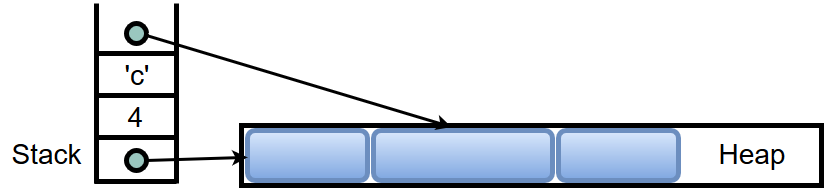
\includegraphics[width=.8\textwidth]{Illustrations/stack_and_heap.png}
\end{center}

\end{frame}

\begin{frame}

\frametitle{GC Cycle}

\emph{Set Condemnation}: determine which objects are garbage 

\linespace
\linespace

\emph{Compaction}: reclaim memory while fighting heap fragmentation

\linespace
\linespace
\linespace

% Don't mention root-level, global objects. Just say objects reached by chaining references from main.
Set condemnation done by \emph{tracing}
\begin{itemize}
\item Detect all reachable objects by chaining references
\end{itemize}

\end{frame}

\begin{frame}

\frametitle{Compaction}

% Need to mention here how to-space and from-space can actually have some areas of memory in common. They are not always distinct places.

Consists of two steps
\begin{itemize}
\item \emph{Relocation}: move objects 
\begin{itemize}
\item \emph{from-space} and \emph{to-space}
\end{itemize}
\item \emph{Remapping}: update object references
\end{itemize}

\linespace

%Make sure to point out that this is the heap.
\begin{center}
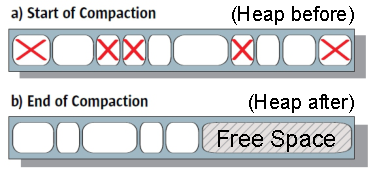
\includegraphics[width=.60\textwidth]{Illustrations/bg_compaction.pdf}
\end{center}

% The compaction process will be our focus, but we want it done concurrently. In order to know what that means though, we need to understand a bit about parallel processing.

\end{frame}



\subsection[PP Basics]{Parallel Processing}

\begin{frame}

\frametitle{Processes and Threads}

\begin{columns}
\begin{column}{0.7\textwidth}

\emph{Process}: instance of a program being run
\begin{itemize}
\item Has its own memory space
\item Examples: JVM, word processor
\end{itemize}

\linespace
\linespace

\emph{Thread}: sequence of independent instructions that can run on its own
\begin{itemize}
\item Component of a process
\item Possible to run multiple in parallel
\end{itemize}

\linespace
\linespace

\emph{Parallel Processing}: running multiple threads simultaneously with multiple processors

\end{column}

\begin{column}{0.30\textwidth}

\begin{center}
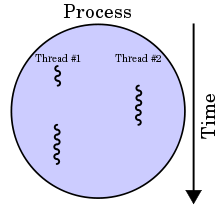
\includegraphics[width=1.0\textwidth]{Illustrations/multithreading.png} \\
{\small \url{wikipedia.org/wiki/Thread_\%28computing\%29}}
\end{center}

\end{column}
\end{columns}

\end{frame}

\begin{frame}

\frametitle{Synchronization}

\only<1>{

\begin{columns}
\begin{column}{0.65\textwidth}
Threads do not communicate

\linespace
\linespace

% Possibly beef up this example later.
Poses new challenges
\begin{itemize}
\item Example: losing object modifications
\end{itemize}

\linespace
\linespace

Need to keep threads synchronized
\end{column}

\begin{column}{0.3\textwidth}

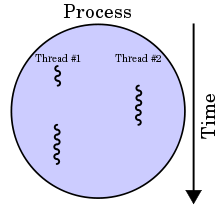
\includegraphics[width=1.0\textwidth]{Illustrations/multithreading.png}

\end{column}
\end{columns}

}

\only<2>{

\emph{Read Barrier}: instructions to run before a thread accesses memory

\linespace
\linespace
\linespace

\begin{center}
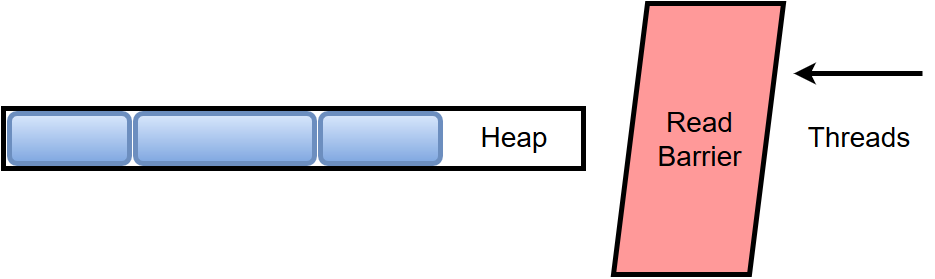
\includegraphics[width=.70\textwidth]{Illustrations/read_barrier.png}
\end{center}

}

\end{frame}



\subsection[GC with PP]{Garbage Collection with Parallel Processing}

\begin{frame}

\frametitle{Concurrency}

We distinguish between application threads and GC threads

\linespace
\linespace

\emph{Concurrent GC}: collector runs at the same time as the application
\begin{itemize}
\item Does not stop the world
\end{itemize}

\linespace
\linespace

Our focus: concurrent compaction!

\end{frame}

\begin{frame}

\frametitle{Latency}

\emph{Latency}: measure of negative impact from GC on application threads
\begin{itemize}
\item Decrease in time spent processing application due to GC
\end{itemize}

\linespace
\linespace

Example: me trying to multi-task

\linespace
\linespace

Many different ways to measure

\linespace
\linespace

Common assessment of concurrent collector performance
%Mention there are other measures, but all my collectors test latency.

\end{frame}



\section[C4]{Continuously Concurrent Compacting Collector (C4)}

\begin{frame}

\frametitle{Continuously Concurrent Compacting Collector (C4)}

\begin{center}
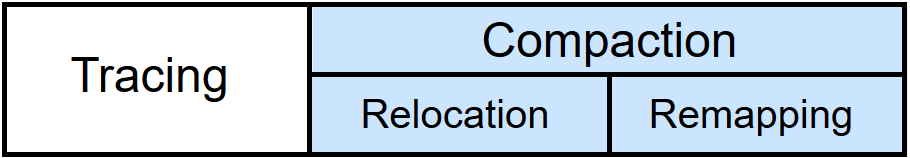
\includegraphics[width=.85\textwidth]{Illustrations/gc_cycle_locator_compaction.png}
\end{center}

\end{frame}



\subsection*{Explanation}

\begin{frame}

\frametitle{Loaded Value Barrier (LVB)}

%Mention that this is during compaction!
Read barrier protects from-space from application threads

\linespace
\linespace

Rule: application can only use moved objects
\begin{itemize}
\item If a thread breaks this, the barrier will correct the situation
\end{itemize}

\linespace
\linespace

This facilitates concurrent relocation and remapping

\end{frame}

\begin{frame}

\frametitle{Concurrent Relocation}

\only<1>{

GC threads simply relocate objects

\linespace
\linespace

All references point to from-space!
\begin{itemize}
\item Application threads certain to trigger LVB
\end{itemize}

\linespace

\begin{center}
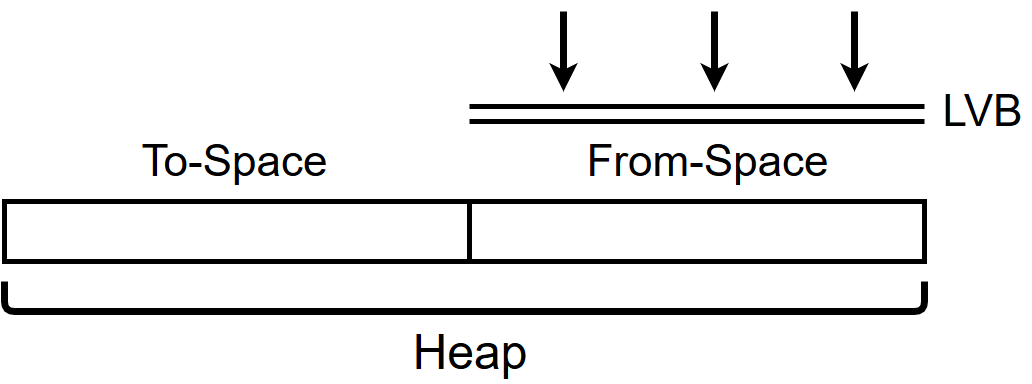
\includegraphics[width=.80\textwidth]{Illustrations/c4_lvb_relocation.png}
\end{center}

}

\only<2>{

How application threads cope
\begin{itemize}
\item If the object was moved, find it
\item If the object is being moved, wait
\item If the object is unmoved, move it
\end{itemize}

\linespace
\linespace

In all cases, correct the reference after

}

\end{frame}

\begin{frame}

\frametitle{Concurrent Remapping}

\only<1>{
\emph{Lazy Remapping}: application threads update references through LVB
\begin{itemize}
\item "If the object was moved, find it"
\item Correct the reference after
\end{itemize}

\linespace
\linespace

To update all references, need to traverse all reachable ones

\linespace
\linespace

Combine remapping with next tracing phase
}

\only<2>{
Remapping combined with tracing
\begin{center}
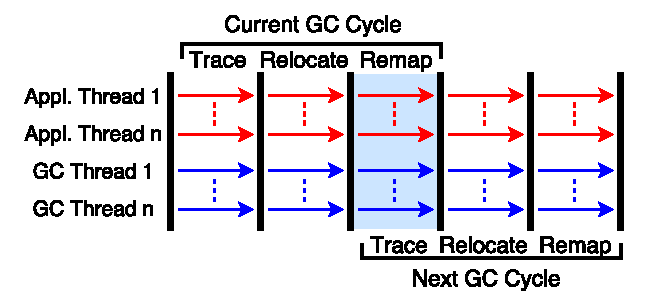
\includegraphics[width=.9\textwidth]{Illustrations/c4Mapping_rough_figure_4.pdf}
\end{center}
}

\end{frame}



\subsection*{Test Results}

\begin{frame}

\frametitle{Testing Environment}

Tested against three garbage collectors
\begin{itemize}
\item Modified version of C4
\item Two algorithms with non-concurrent compaction
\end{itemize}

\linespace
\linespace

Improvements from concurrent compaction

\end{frame}

\begin{frame}

\frametitle{Results}

%Show the figures from the paper here and start talking about them
%\only<1>{
%\begin{center}
%Application Worst Case Response Times
%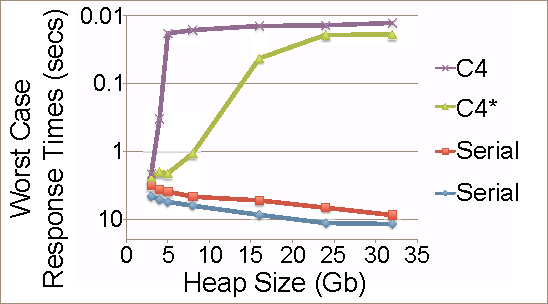
\includegraphics[width=.80\textwidth]{Illustrations/c4_results.pdf}
%\end{center}
%}

%\only<2>{
\begin{columns}
\begin{column}{0.5\textwidth}

\color[RGB]{135,35,142}C4\color{black}:
\begin{itemize}
\item Has fastest response times
\item Maintains them for largest range of heap sizes
\item Least impact on application
\end{itemize}

\linespace
\linespace

Priority given to GC threads

\linespace
\linespace

Still has best application responsiveness

\end{column}

\begin{column}{0.5\textwidth}
\begin{center}
Worst Case Response Times
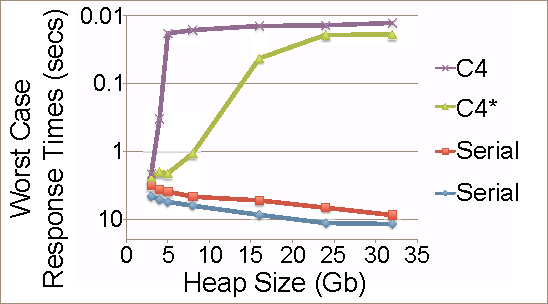
\includegraphics[width=.89\textwidth]{Illustrations/c4_results.pdf}
\end{center}
\end{column}
\end{columns}
%}

\end{frame}



%\section[Collie]{Collie Collector}
%
%\begin{frame}
%
%\frametitle{Collie Garbage Collector}
%
%\begin{center}
%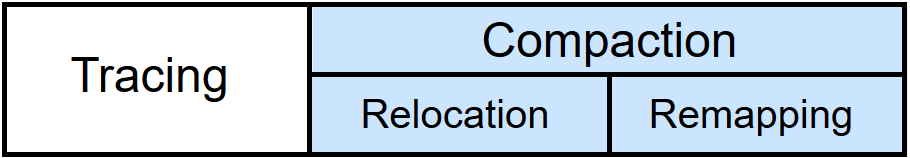
\includegraphics[width=.85\textwidth]{Illustrations/gc_cycle_locator_compaction.png}
%\end{center}
%
%\end{frame}
%
%
%
%\subsection*{Explanation}
%
%\begin{frame}
%
%\frametitle{Transactions}
%
%%Remember to emphasize the key point is interruptions will cause nothing to happen, or everything to.
%\emph{Transaction}: series of operations performed in an all-or-none manner
%
%\linespace
%\linespace
%
%Example: updating prices in a store for sales \\
%\begin{itemize}
%\item Update sale price
%\item Update store price
%\end{itemize}
%
%\linespace
%\linespace
%
%Protects data from interrupts
%
%%\linespace
%%\linespace
%%
%%\emph{Transactional Memory}: allows code sections to run like transactions
%%\begin{itemize}
%%\item Memory used by the code is protected
%%\end{itemize}
%
%\end{frame}
%
%\begin{frame}
%
%\frametitle{Transplantations}
%
%\emph{Transplantation}: relocating and remapping objects
%
%\linespace
%\linespace
%
%\begin{columns}
%\begin{column}{0.33\textwidth}
%
%Transaction:
%\begin{itemize}
%\item Start transaction
%%\item Check object
%\item Relocate object
%\item Remap references
%\item End Transaction
%\end{itemize}
%
%\end{column}
%\begin{column}{0.32\textwidth}
%
%$\xrightarrow{\text{Interrupted by application}}$
%
%\end{column}
%\begin{column}{0.3\textwidth}
%
%Mark object as \emph{non-individually transplantable} (NIT)
%
%\end{column}
%\end{columns}
%
%\end{frame}
%
%\begin{frame}
%%either cut talking about the details or mention that heap is virtual memory earlier.
%
%\frametitle{Leftovers}
%
%\begin{columns}
%\begin{column}{0.5\textwidth}
%What happens to NIT objects?
%
%\linespace
%\linespace
%
%Lie to the compactor
%\begin{itemize}
%\item Mirrored-to-space
%\item Zero-copy transplantation
%\end{itemize}
%
%\linespace
%\linespace
%
%\emph{Aborting Compactor}: no progress guarantees
%\end{column}
%\begin{column}{0.5\textwidth}
%
%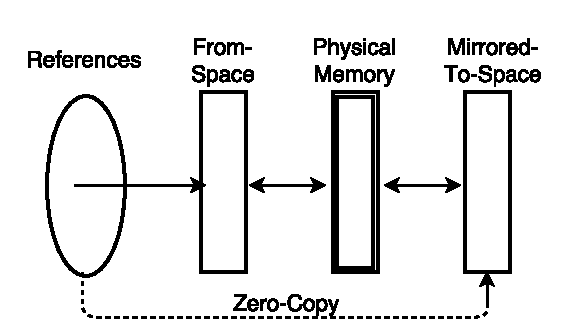
\includegraphics[width=.95\textwidth]{Illustrations/collie_mirrored_rough.pdf}
%
%\end{column}
%\end{columns}
%
%\end{frame}
%
%
%
%\subsection*{Test Results}
%
%\begin{frame}
%
%\frametitle{Testing Environment}
%
%Tested against the Pauseless Garbage Collector
%\begin{itemize}
%\item Ancestor of Collie
%\item Largely concurrent with some stop-the-world pauses
%\item Also requires supportive hardware
%\end{itemize}
%
%\linespace
%\linespace
%
%Standard JVM benchmarks used to test latency
%\begin{itemize}
%\item Improvements from aborting nature and transactions
%\end{itemize}
%
%\end{frame}
%
%\begin{frame}
%
%\frametitle{Results}
%
%\only<3>{
%\begin{center}
%Minimum Mutator Utilization (MMU) Percentages \\for Various Time Windows\\
%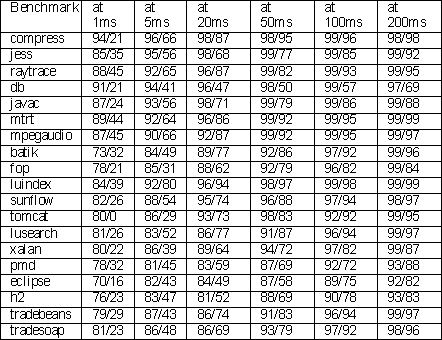
\includegraphics[width=.65\textwidth]{Illustrations/collie_results.pdf}
%\end{center}
%}
%
%\only<1>{
%\begin{center}
%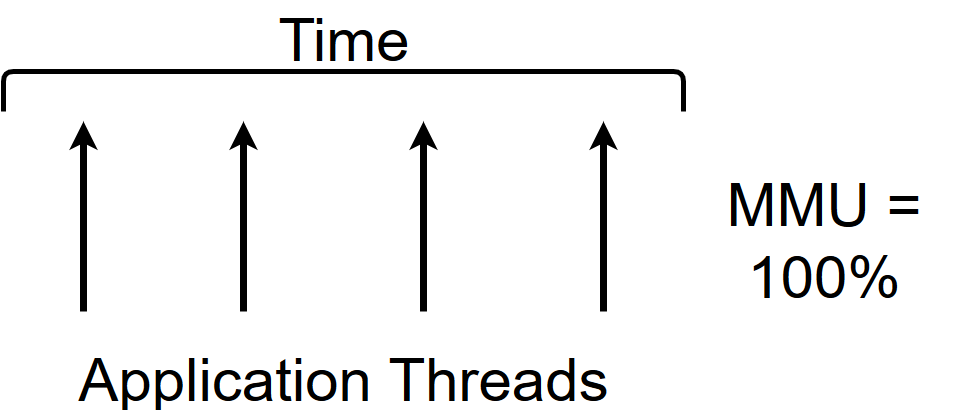
\includegraphics[width=.80\textwidth]{Illustrations/collie_mmu_explanation_1.png}
%\end{center}
%}
%
%\only<2>{
%\begin{center}
%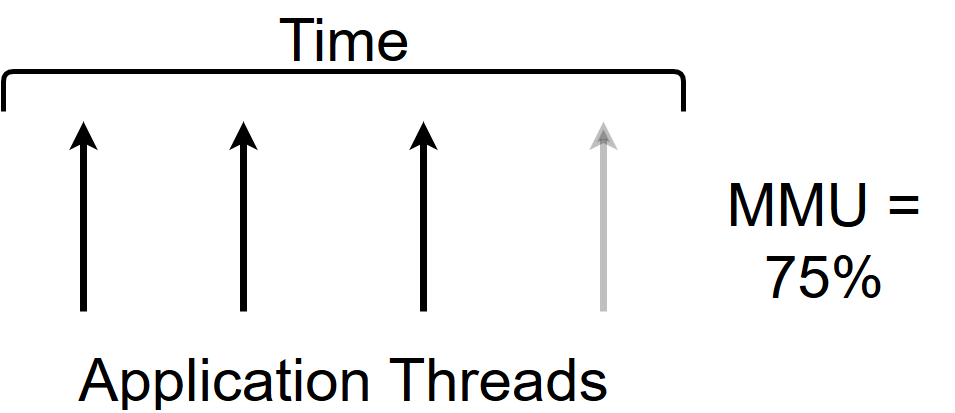
\includegraphics[width=.80\textwidth]{Illustrations/collie_mmu_explanation_2.png}
%\end{center}
%}
%
%\only<4>{
%\begin{columns}
%\begin{column}{0.5\textwidth}
%
%\color{red}Collie \color{black}has higher MMU than \color{blue}Pauseless \color{black}across the board
%\begin{itemize}
%\item Application threads used more
%\end{itemize}
%
%\linespace
%\linespace
%
%Application threads have priority over GC threads
%
%\linespace
%\linespace
%
%Lends itself well to latency but no progress guarantees
%
%\end{column}
%
%\begin{column}{0.5\textwidth}
%\begin{center}
%MMU Percentages
%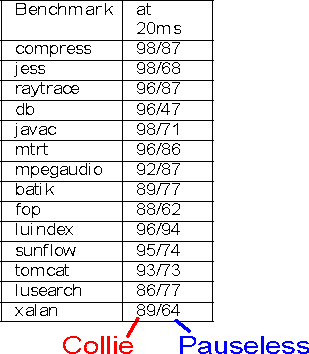
\includegraphics[width=.90\textwidth]{Illustrations/collie_results_2.pdf}
%\end{center}
%\end{column}
%\end{columns}
%}
%
%\end{frame}



\section[FPP]{Field Pinning Protocol}

\begin{frame}

\frametitle{Field Pinning Protocol (FPP)}

\begin{center}
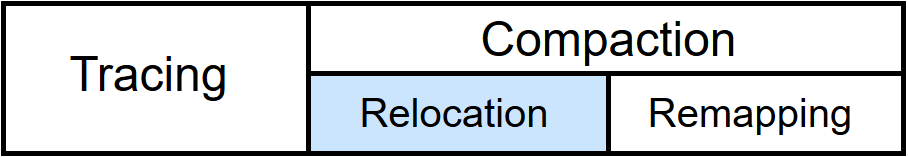
\includegraphics[width=.85\textwidth]{Illustrations/gc_cycle_locator_relocation.png}
\end{center}

\end{frame}



\subsection*{Explanation}

\begin{frame}

\frametitle{Hazard Pointers}

\emph{Hazard Pointers}: values that show which objects an application thread is accessing
\begin{itemize}
\item \emph{Pin} the object
\end{itemize}

\linespace
\linespace

Inform other threads of objects that are in use

\linespace
\linespace

Main goal: safely access objects without worrying about relocation

%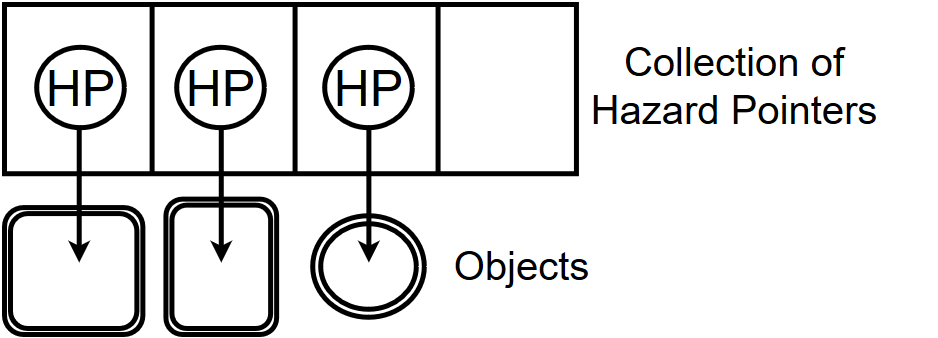
\includegraphics[width=.95\textwidth]{Illustrations/FPP_HP_Illustration.png}


\end{frame}


\begin{frame}

\frametitle{Example}

\begin{columns}
\begin{column}{0.45\textwidth}
	\begin{itemize}
	\item Object = Coffee 
	\item \color{red}{Application Thread = Person w/ Coffee Cup} 
	\only<2->{\item \color{blue}{Relocation Thread = Person}}
	\only<2->{\item \color{black}{* = Responsible}} 
	\only<2->{\item ! = Impeded}
	\end{itemize}
\end{column}
\begin{column}{0.55\textwidth}
	\only<1>{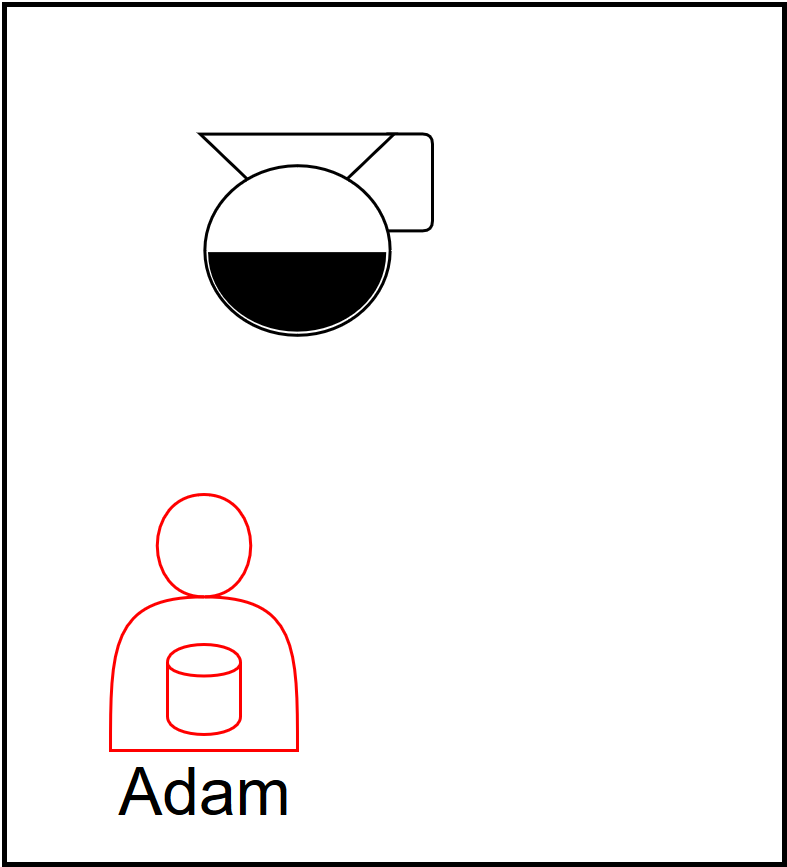
\includegraphics[width=.95\textwidth]{Illustrations/coffeeLineNew1.png}}
	\only<2>{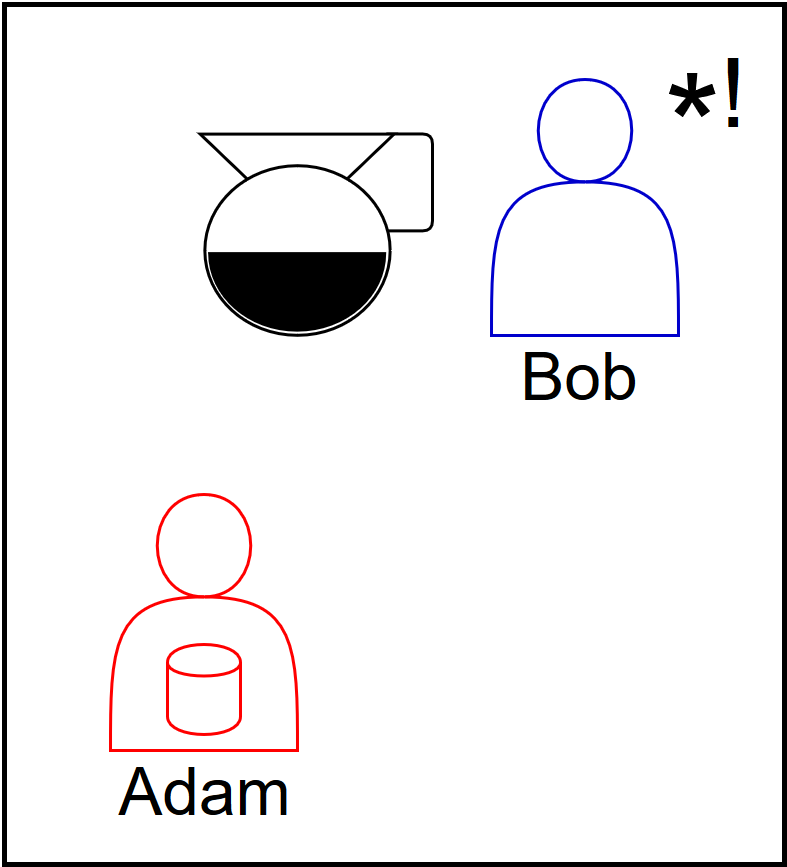
\includegraphics[width=.95\textwidth]{Illustrations/coffeeLineNew2.png}}
	\only<3>{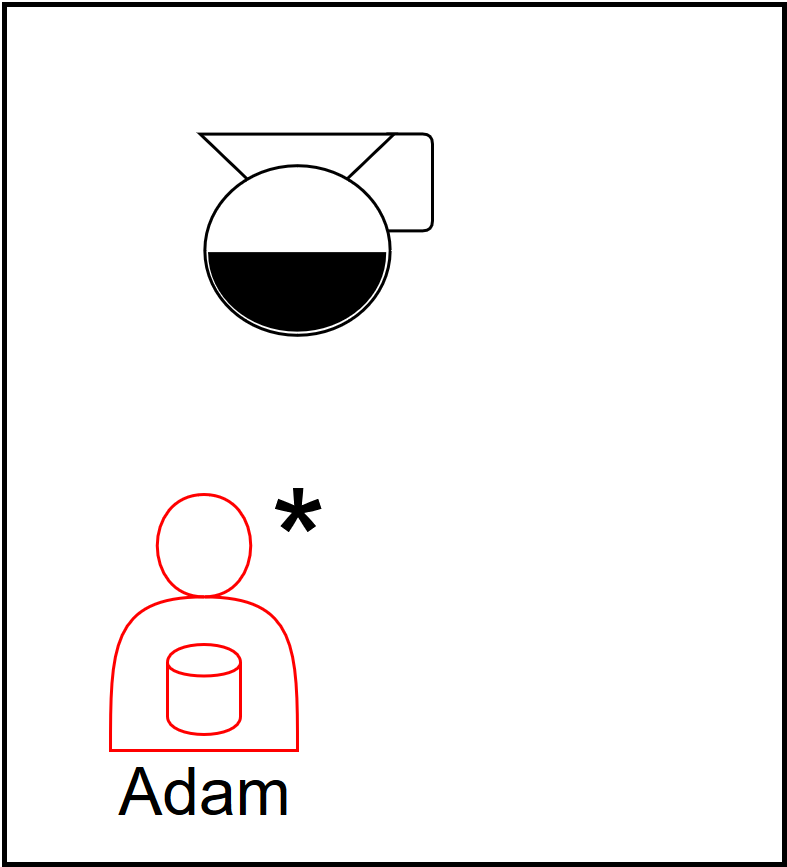
\includegraphics[width=.95\textwidth]{Illustrations/coffeeLineNew3.png}}
	\only<4>{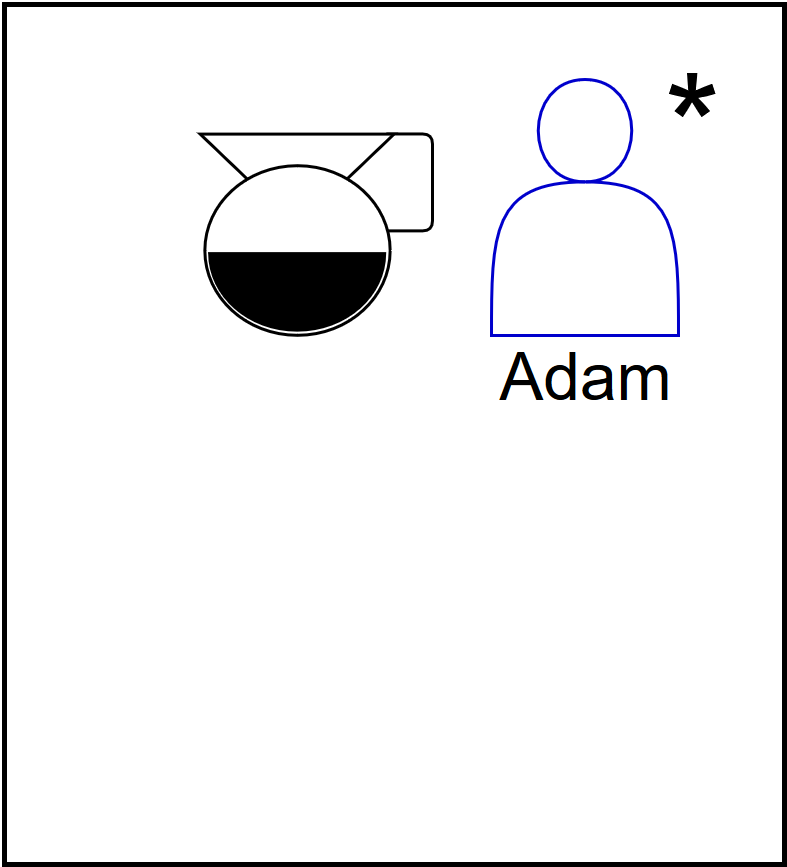
\includegraphics[width=.95\textwidth]{Illustrations/coffeeLineNew4.png}}
	\only<5>{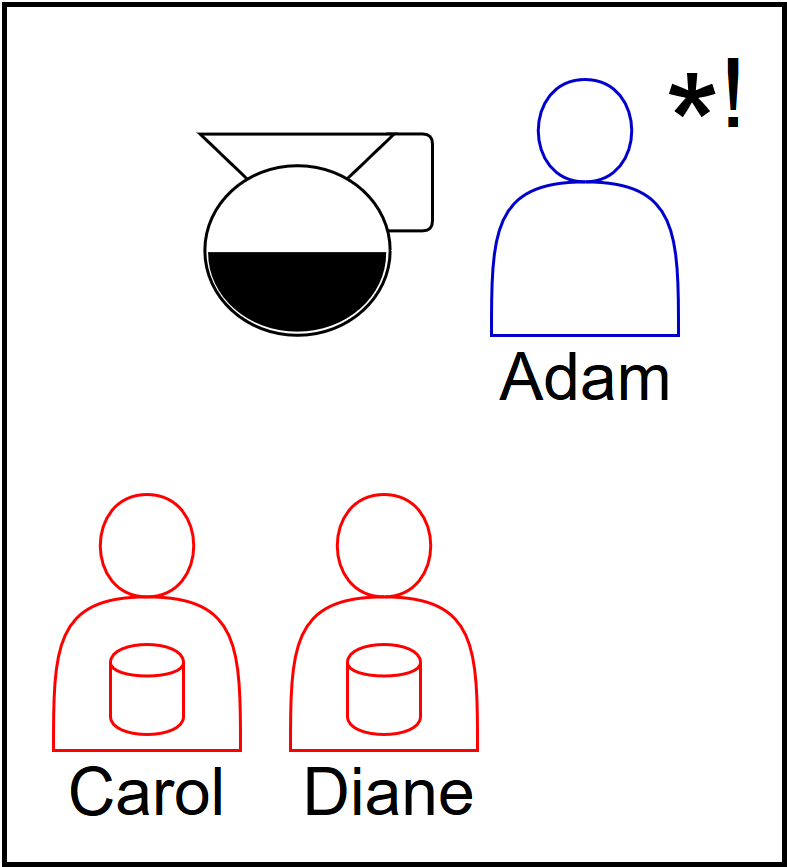
\includegraphics[width=.95\textwidth]{Illustrations/coffeeLineNew5.png}}
\end{column}
\end{columns}

\end{frame}


\begin{frame}

\frametitle{Concurrent Relocation through Blame}

%If time allows and feedback demands, could break this into multiple slides to not have so much text
%on one as well as to refer back to the example and characters more.

\emph{Blamed Thread}: responsible for relocating an object
\begin{itemize}
\item Comes from hazard pointers (coffee cups) impeding copying
\end{itemize}

\linespace
\linespace

Relocation with FPP
\begin{itemize}
\item GC threads attempt to relocate objects
\item Impeding application threads are blamed
\begin{itemize}
\item When finished with the object, try to move
\end{itemize}
\item Blame passed to impeding threads until relocation succeeds
\end{itemize}

\end{frame}


%\begin{frame}
%
%\frametitle{An Application Thread's Perspective}
%
%Process followed by an \color{red}{application thread}\color{black}
%\linespace
%
%\begin{columns}
%\begin{column}{0.5\textwidth}
%\begin{enumerate}
%\item Pin object with a hazard pointer
%\item Check if the object has been moved already
%\item Use the object without worry
%\item Unpin the object when done
%\item If blamed, try to relocate the object
%\end{enumerate}
%\end{column}
%
%\begin{column}{0.5\textwidth}
%\begin{enumerate}
%\item Get a coffee cup
%\item Check that the coffee is still in the room
%\item Drink all the coffee you want
%\item Discard your coffee cup
%\item If blamed, try to move the coffee
%\end{enumerate}
%\end{column}
%\end{columns}
%
%\end{frame}



\subsection*{Test Results}

\begin{frame}

\frametitle{Testing Environment}

Implemented in the Garbage-First (G1) Garbage Collector
\begin{itemize}
\item Concurrent tracing and remapping
\item Relocation requires stop-the-world pauses
\end{itemize}

\linespace
\linespace

Tested against the default G1 collector

\linespace
\linespace

Improvements from solely concurrent relocation

\end{frame}

\begin{frame}

\frametitle{Results}

%Show the figures from the paper here and start talking about them
%\only<1>{
%\begin{center}
%Average GC Pauses for Various Benchmarks
%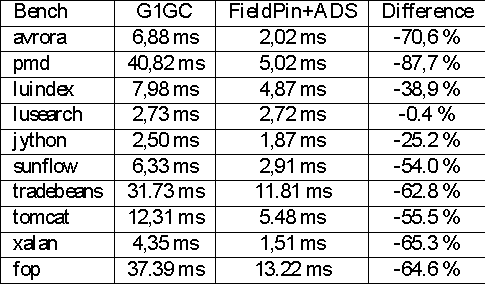
\includegraphics[width=.80\textwidth]{Illustrations/fpp_results.pdf}
%\end{center}
%}

%\only<2>{
\begin{columns}
\begin{column}{0.5\textwidth}

\color{red}G1 with FPP \color{black}on average 50\% shorter pauses than \color{blue}standard G1\color{black}
\begin{itemize}
\item Less impact on application thread performance
\end{itemize}

\linespace

Most latency from host activities

\linespace

Priority given to application threads

\linespace

Concurrent relocation without barriers is feasible

\end{column}

\begin{column}{0.5\textwidth}
\begin{center}
Average GC Pauses
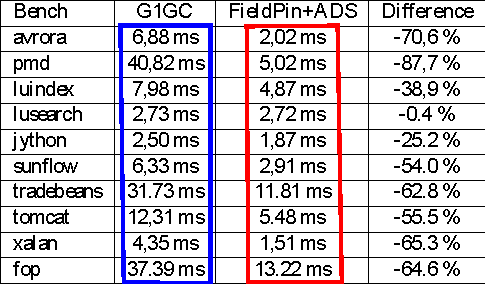
\includegraphics[width=.90\textwidth]{Illustrations/fpp_results_2.pdf}
\end{center}
\end{column}
\end{columns}
%}

\end{frame}



\section[Conclusions]{Conclusions}

%\begin{frame}
%
%\frametitle{Breaking Down Barriers}
%
%Moving toward concurrent compaction without barriers
%\begin{itemize}
%\item C4 - heavily relies on barriers
%\item FPP - barrier-free
%\end{itemize}
%
%\linespace
%\linespace
%
%No barriers are desirable as they add overhead
%
%\end{frame}

\begin{frame}

\frametitle{Conclusions}

Moving toward concurrent compaction without barriers
\begin{itemize}
\item C4 - heavily relies on barriers
\item FPP - barrier-free
\end{itemize}

\linespace
\linespace

Different approaches to prioritizing GC vs application
\begin{itemize}
\item C4 - focus on GC
\item FPP - focus on application
\end{itemize}

\linespace
\linespace

Tough to compare them directly

\linespace
\linespace

All tests showed that concurrency can improve latency
\begin{itemize}
\item Approach used will depend on intended environment
\end{itemize}

\end{frame}

\begin{frame}
	\frametitle{Thanks for your time!}
	
	\begin{center}
	{\huge Questions?}
	\end{center}	
	
	\linespace
	\linespace	
	
	\begin{center}
	Contact: opdah023@morris.umn.edu
	\end{center}
	
\end{frame}



\section*{References}

\begin{frame} 
	\frametitle{References} 
	
%	\begin{thebibliography}{lskdjf}
%	
%	\bibitem{McPhee:2009:gecco}
%N.~F. McPhee, E.~Crane, S.~Lahr, and R.~Poli.
%\newblock Developmental Plasticity in Linear Genetic Programming.
%\newblock In G\"unther Raidl, \emph{et al}, editors, {\em GECCO '09}, pages 1019--1026, Montr\'eal, Qu\'ebec, Canada, 2009.
%	
%	\bibitem{citeulike:3452411}
%	R.~Poli and N.~McPhee.
%\newblock A linear estimation-of-distribution {GP} system.
%\newblock In M.~O'Neill, \emph{et al}, editors, {\em EuroGP 2008}, volume
%  4971 of {\em LNCS}, pages 206--217, Naples,
%  26-28 Mar. 2008. Springer.
%  
%  	\end{thebibliography}
%	
%	\linespace
%	\begin{center}
%	See the GECCO '09 paper for additional references.
%	\end{center}

\begin{thebibliography}{lskdjf}

\bibitem{Lowe:2015}
E.~\"{O}sterlund and W.~L\"{o}we.
\newblock Concurrent compaction using a field pinning protocol. 
\newblock 2015 ACM SIGPLAN International Symposium on Memory Management (ISMM 2015). ACM, New York, NY, USA, 56-69.

\bibitem{Tene:2011}
G.~Tene, B.~Iyengar, and M.~Wolf.
\newblock C4: the continuously concurrent compacting collector.
\newblock 2011 ACM SIGPLAN International Symposium on Memory Management (ISMM 2011). ACM, New York, NY, USA, 79-88.

\bibitem{Iyengar:2012}
B.~Iyengar, G.~Tene, M.~Wolf, and E.~Gehringer.
\newblock The Collie: a wait-free compacting collector.
\newblock 2012 ACM SIGPLAN International Symposium on Memory Management (ISMM 2012). ACM, New York, NY, USA, 85-96.

\linespace
\begin{center}
\color{black}See the UMM Opdahl Fall '15 paper for additional references.
\end{center}


\end{thebibliography}

\end{frame} 



\end{document}


